\chapter{Persistence}
In the world of data we rarely have a topological description of the space our dataset lives in. We could endow our the space which our data lives in with a topology, but just giving it the discrete topology the homology of that space would not be very informative.

What if there is an underlying topological space with a non trivial topology? Consider for example the points sampled from an annulus in Figure \ref{annulus:points}.

\begin{figure}[ht]
  \centering
  \begin{subfigure}[t]{.5\linewidth}
    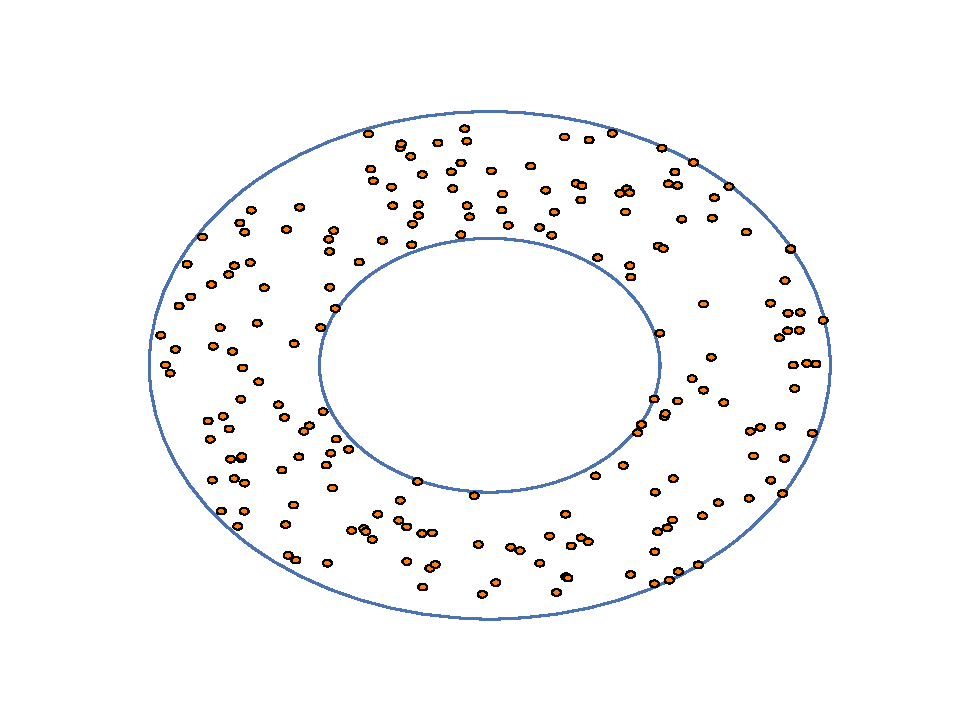
\includegraphics[scale=.5]{annulus.pdf}
    \caption{\label{annulus:points}}
 \end{subfigure}%
  \begin{subfigure}[t]{.5\linewidth}
    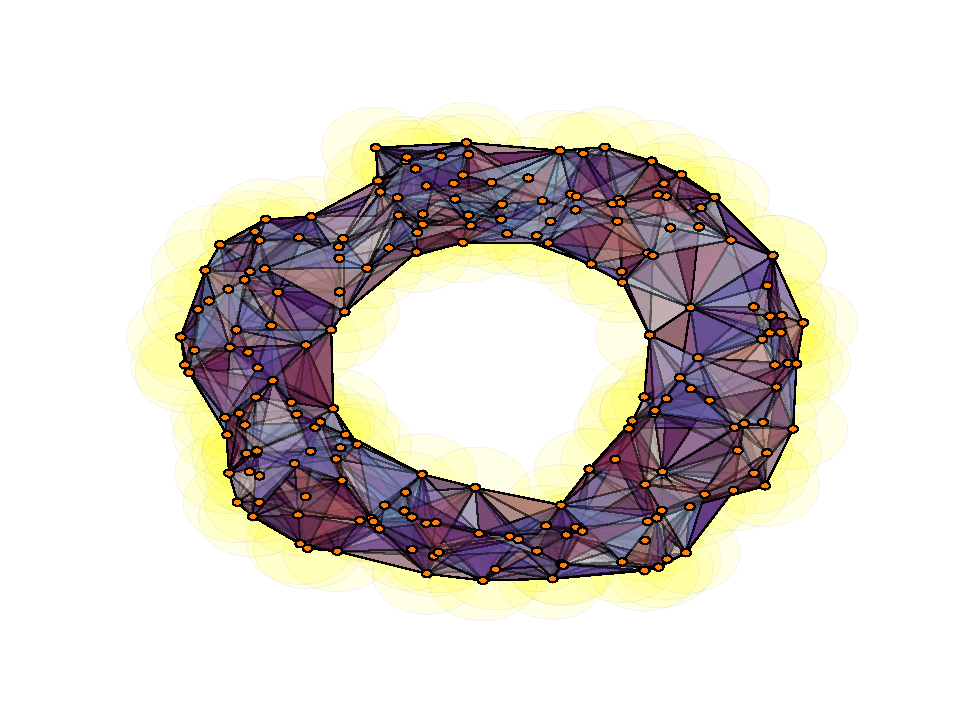
\includegraphics[scale=.5]{annulus_rips.pdf}
    \caption{\label{annulus:imposed}}
 \end{subfigure}
  \caption{\label{annulus} Imposing a simplicial complex \textbf{(b)} on data sampled from an annulus \textbf{(a)}.}
\end{figure}


If we know our space is an annulus we know what the homology is of this space, it contains a single cycle, but with raw data (figure without annulus) this can be harder to tell. This is where persistent homology comes in, a way of gaining information about the homological structure of the data space.

The basic idea is quite simple. Using the theory of simplicial homology we can impose an abstract simplicial complex on our dataset as in Figure \ref{annulus:imposed}. A natural way of doing this is defining some form of metric on our space, not necessarily metric in the sense of a metric space, such that when points are sufficiently close to each other we say they belong to the same simplex.

However, there is a problem with the idea in its naive form. How large is ``sufficiently close''? If we use too large of a distance we end up with all points in a single simplex and retrieve no valuable homological information. On the other hand, if the distance is too small we end up with a simplicial complex with very few connections between vertices and this too could prove uninformative. Persistent homology addresses this by simply considering \textit{all} of them and encoding the lifetime of homological features occuring in something called a \textit{barcode diagram}.

% First we need to recall the definition of a homotopy. A homotopy between to continuous maps $f,g$ is another continous map $H: X \times [0,1] \to Y$ such that $H(-,0) = f$ and $H(-,1) = g$. This defines an equivalence relation and we say that $f \simeq g$ meaning that $f$ is homotopy equivalent to $g$.

% We say two topological spaces $X,Y$ are homotopy equivalent, and hence overloading the meaning of this expression, when there exists continuous maps $f: X \to Y$ and $g: Y \to X$ such that $g \circ f \simeq id_{X}$  and $f \circ g \simeq id_{Y}$. This gives an equivalence relation on topological spaces and we write $X \simeq Y$ to mean that they have the same homotopy type.

% After this brief detour we can now look at nerves. We define the nerve of a finite collection of sets to be
% \[nrv(K) = \{ X \subseteq K \mid \bigcap X \neq \emptyset \}\]

% Nerve theorem. Let $F$ be a finite collection of closed convex sets in Euclidean space. Then the nerve of F and the union of the sets in F have the same homotopy type.

\section{Filtrations}
The perhaps most natural way to impose an abstract simplicial complex on a set of points is the Cech complex
\begin{definition}[Cech complex]
For a given selection of points $\{x_{\alpha}\}$ in some Euclidean space $\mathbb{R}^{n}$ the Cech complex $C_{\epsilon}$ is given by the abstract simplicial complex whose $k$-simplices are given by $k+1$ points in the collection of points whose closed balls of radius $\epsilon/2$ have a point in common.
\end{definition}

The Cech complex is a special case of something called the nerve of a topological space. Through the Nerve theorem (cite) this guarantees that the Cech complex has the same homotopy type as the underlying space given some assumptions (what are they?). A well known result in algebraic topology is that if two spaces have the same homotopy type, they in particular have the same homology groups (cite).

However, the Cech complex is for practical purposes not feasible to compute (cite). The reason being that we need to keep the entire simplicial complex in memory and this can be quite expensive (elaborate this).

A sort of compromise is the Vietoris-Rips complex as seen in Figure \ref{manyrips}. This complex is a simplification where we do not look for points in common, but rather say that if $k+1$ vertices intersect pairwise they form a $k$-simplex.

\begin{figure}
  \centering
  \begin{subfigure}[t]{.5\linewidth}
    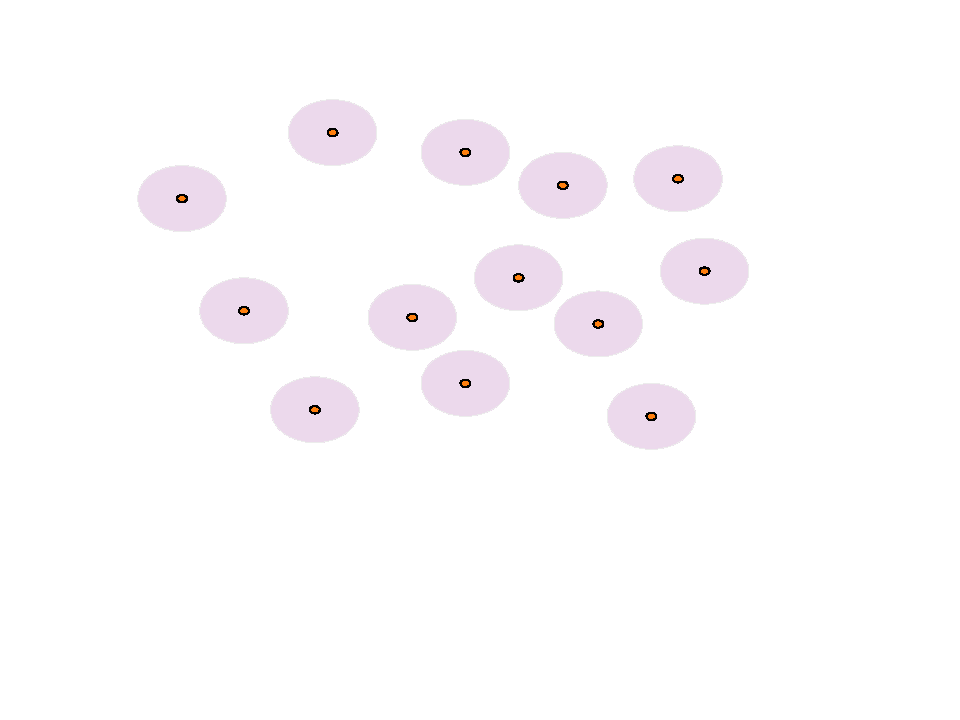
\includegraphics[scale=.5]{rips_eps=01.pdf}
    \caption{$\epsilon=0.1$}
 \end{subfigure}%
  \begin{subfigure}[t]{.5\linewidth}
    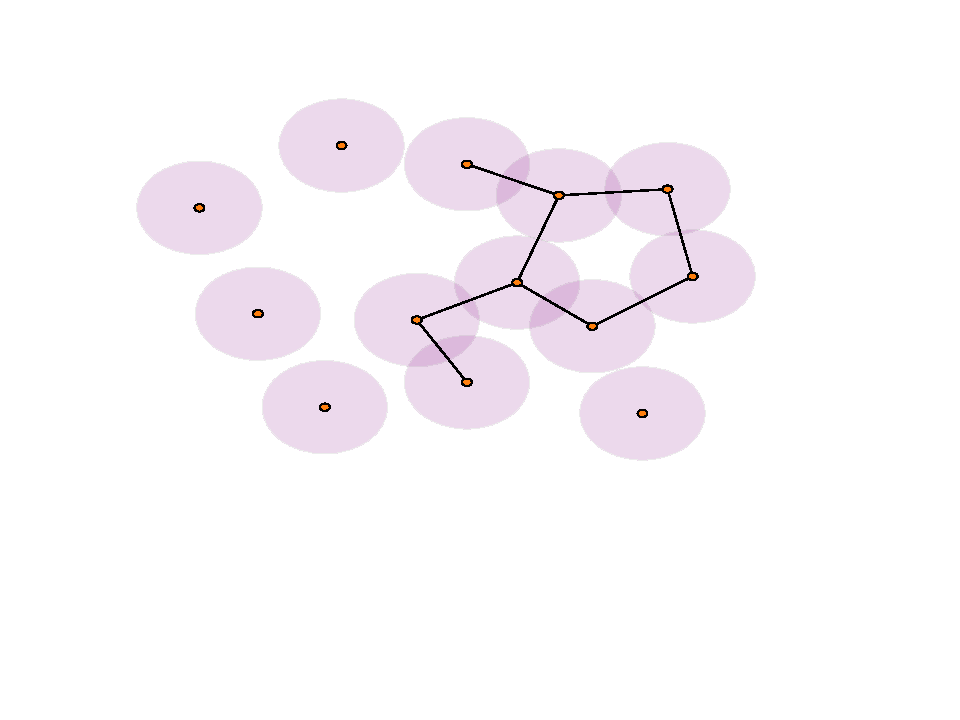
\includegraphics[scale=.5]{rips_eps=015.pdf}
    \caption{$\epsilon=0.15$}
 \end{subfigure}
  \begin{subfigure}[b]{.49\linewidth}
    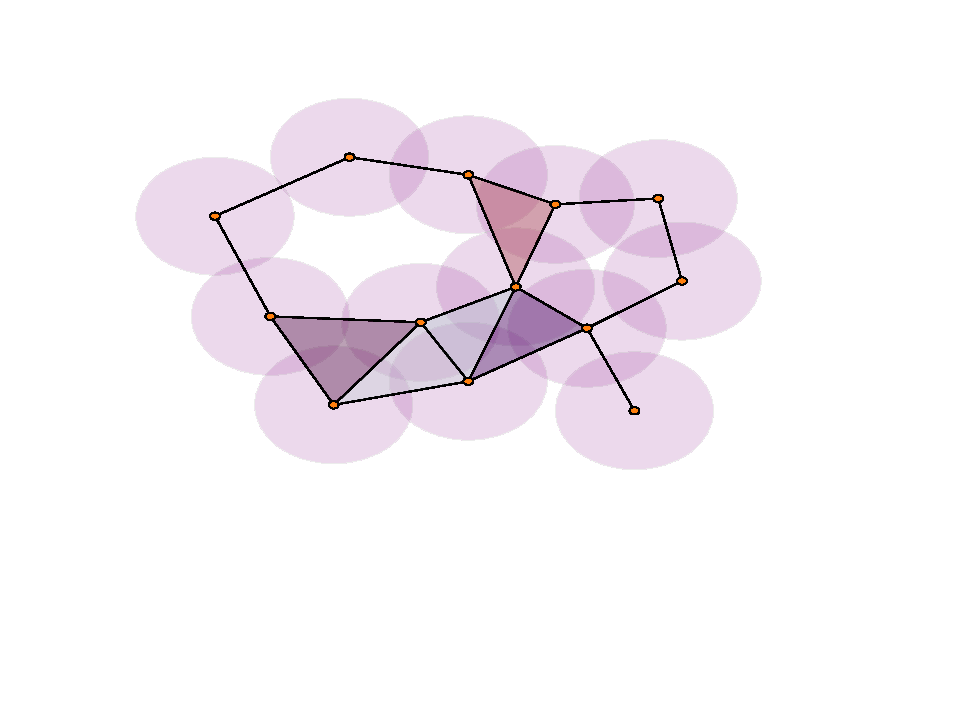
\includegraphics[scale=.5]{rips_eps=02.pdf}
    \caption{$\epsilon=0.2$}
 \end{subfigure}
  \begin{subfigure}[b]{.5\linewidth}
    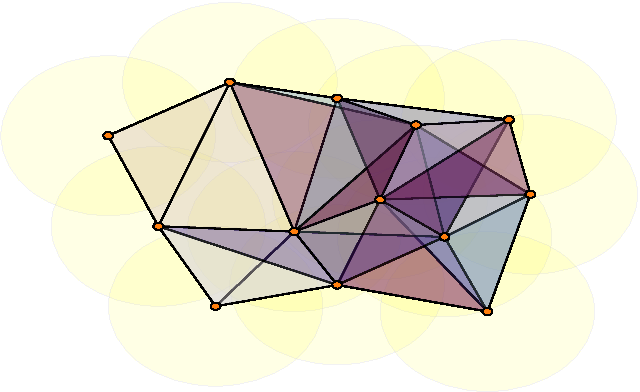
\includegraphics[scale=.5]{rips_eps=03.pdf}
    \caption{$\epsilon=0.3$}
 \end{subfigure}
 \caption{The Vietoris-Rips complex at different $\epsilon$-values.}
 \label{manyrips}
\end{figure}
\begin{definition}[Vietoris-Rips complex]
For a given selection of points $\{x_{\alpha}\}$ in some Euclidean space $\mathbb{R}^{n}$ the Vietoris-Rips complex $R_{\epsilon}$ is the abstract simplicial complex whose $k$-simplices are given by $k+1$ points which are pairwise at most $\epsilon$ apart.
\end{definition}

The Vietoris-Rips complex does not come with the same guarantee if fidelity to the underlying space as the Cech complex does. However, it is entirely defined by the vertices and the edges of the simplicial complex, allowing it to be stored as a simple graph (elaborate why the edges and vertices are enough).

Given a monotonically increasing sequence of resolutions $(\epsilon_{i})_{i \in I}$ we can associate to a finite set of points $X$ the Vietoris-Rips complexes $(R_i)_{{i \in I}}$. Then there are natural inclusions:
\begin{center}
\begin{tikzcd}
R_1 \arrow[hookrightarrow]{r}{x} & R_2 \arrow[hookrightarrow]{r}{x} & \dots \arrow[hookrightarrow]{r}{x} & R_{n-1} \arrow[hookrightarrow]{r}{x} & R_n
\end{tikzcd}
\end{center}
We then look at the image of the induced inclusions $x: H_{*}(R_{i}) \to H_{*}R_{j}$ where $i < j$. These inclusions tell us what homological features persist going from resolution $\epsilon_{i}$ to resolution $\epsilon_{j}$.

This lends some credibility to the Vietoris-Rips construction as an approximation of the underlying space since it establishes a relationship between it and the Cech complex through a result due to de Silva (cite).
\begin{lemma}
  Given $\epsilon > 0$ there is a chain of inclusions
  \[R_{\epsilon} \hookrightarrow C_{\epsilon \sqrt{2}} \hookrightarrow R_{\epsilon \sqrt{2}}\]
\end{lemma}
This tells us that any feature preserved in the inclusion $R_{\epsilon} \to R_{\epsilon \sqrt{2}}$ is also present in the Cech complex at resolution $\epsilon \sqrt{2}$ and so in the underlying topological space by theorem ?. In fact, any feature that is preserved up to resolution $\epsilon'\geq \epsilon \sqrt{2}$ is present in the Cech complex at resolution $\epsilon'$.

We are now ready to state formally what persistent homology  is. While the Vietoris-Rips complex is a common used way of approximating a simplicial complex on a data-set we can be more general than that.

\begin{definition}
A \textbf{filtration} of a simplicial complex $K$ is a totally ordered set of subcomplexes $K^{i}  \subseteq K$ for $i \in \mathbb{N}$ such that if $i \leq j$ then $K^{i} \subseteq K^{j}$.
\end{definition}

Note that the Cech and Vietoris-Rips complexes are two instances of filtrations, but with this definition we are not restricted to them alone. This means we can compute persistent homology for \textit{any} filtration.

\begin{definition}
  For $p > 0$ the \textbf{$p$-persistent $k$th homology module} of $K^{i}$ is given as
  \[H^{i,p}_{k} = Z^{i}_{k}/(B^{{i+p}}_{k} \cap Z^{i}_{k})\]
\end{definition}
This module is well-defined since the inclusion $K^{i} \hookrightarrow K^{i+p}$ induces inclusions $K^{i}_{k} \hookrightarrow K_{k}^{i+p}$ hence we have inclusions $Z^{i}_{k} \hookrightarrow K^{i}_{k} \hookrightarrow K_{k}^{i+p}$ and so $Z^{i}_{k}$ is a submodule of $K^{i+p}_{k}$.

Since we can associate each simplicial subcomplex $K^{i}$ in a filtration with a simplicial chain complex $K^{i_{*}}$ we can associate with each filtration a complex of simplicial chain complexes.
\section{Persistence Module}
While we have arrived at a definition (refer) that serves as a sufficient framework for persistent homology, it is still particular in the sense that we are talking about simplicial complexes and filtrations on them. It is possible to make the notion of persistent homology even more general which allows us to understand its algebraic structure even better. This does not mean that we should entirely discard our anchoring of persistent homology in the realm of simplicial complexes, as it relates closely to how we will do persistent homology in practice, but rather we should let this more abstract approach serve as the theoretical underpinning which opens up the possibility of other types of approximation of data than simplicial complexes.

In order to transition from simplicial complexes to a more general framework we need some definitions that has us end up in  a less particular construction of persistent homology.
\begin{definition}[{\cite[p. ~2]{weibel1994}}]
  Let $C_{*},D_{*}$ be chain complexes over some ring $R$. A \textbf{chain map} $u: C_{*} \to D_{*}$ is a family of $R$-module homomorphisms $u_{k}: C_{k} \to D_{k}$ such that the following diagram commutes
  \begin{center}
% https://tikzcd.yichuanshen.de/#N4Igdg9gJgpgziAXAbVABwnAlgFyxMJZARgBoAGAXVJADcBDAGwFcYkQBhAfWAGsBqYgF8QQ0uky58hFACYK1Ok1btuvUeJAZseAkQDMCmgxZtEnHrwC0wjRJ3SiZYopMrzAEUuCRY+1L05UhdjZTMQL3U-LUldGWRDEKVTdi8+G19NbQD48iNk9xAAHSKoCBwEaOy4ojykt3CSsoq7GIdA5AAWfIb2JvLKrNjHFG76sL7SgdFFGCgAc3giUAAzACcIAFskADYaHAgkPILGorR6Nbwmb1lM1Y3txGODpEMT9mZvW2j1raQAdn2h0Qb165hK50uWGufH4t1av0ez2BZHe4LOFyujC+dxAiKQqJeiHkaOKGKhMN4uPxIKBSG6pIhmOh2Nh300NIZRIArKEUujIViuFEOQ8kCSeXzCp90uz7n9iXTEAAOKWnQUsywZBFixC8kBEgCcasmGsp2p+usJwIZYJAnyilCEQA
\begin{tikzcd}
\dots \arrow[r, "\partial_{k+2}"] & C_{k+1} \arrow[d, "u_{k+1}"] \arrow[r, "\partial_{k+1}"] & C_k \arrow[r, "\partial_{k}"] \arrow[d, "u_k"] & C_{k-1} \arrow[d, "u_{k-1}"] \arrow[r, "\partial_{k-1}"] & \dots \\
\dots \arrow[r, "\partial_{k+2}"] & D_{k+1} \arrow[r, "\partial_{k+1}"]                      & D_k \arrow[r, "\partial_k"]                    & D_{k-1} \arrow[r, "\partial_{k-1}"]                      & \dots
\end{tikzcd}
  \end{center}
\end{definition}

\begin{definition}
  A \textbf{persistence complex} is a family of chain complexes $C^{i}_{*}$ together with chain maps $\iota^{i}: C^{i} \to C^{i+1}$ that go between them in the following way
% https://tikzcd.yichuanshen.de/#N4Igdg9gJgpgziAXAbVABwnAlgFyxMJZARgBpiBdUkANwEMAbAVxiRAGkA9YLAXwH1gAawDUxXiF6l0mXPkIoyAJiq1GLNlyyChEqTOx4CRJeVX1mrRB25YxA4fcnSQGQ-JOkV1Cxutceex09Fzc5YxQABjMfdSsQAB0EqAgcBH1XWSMFZGjvNUs2JJS05wNwnLJI8ziihJoS9NCsjxRTatjC6ySG1Kby7KIAZhiCv0TkvrLM9wjkEfzfeOKpjLDBxVIhmq6J3tK1lrnTbc7xnsbJVRgoAHN4IlAAMwAnCABbJDIQHAgkEZ+dCwDDYAAsIBAhCAzssEvgcHR+Fhpq8Pkhoj8-ohvgw6AAjGAMAAKRwUIAYMCeOGhY1haDoLzwjB0TgyqM+iFMmP+MLq9MZWGZjnEKLeHIxvyQXIRwLBEKh1FxBOJpLYFKpNKWdXhdE4yLZYqQABZqJLEBKgSDrODIZrat04alETwALQig1oxAAVlNWO+MqtIBtCtp2qdgiwbpCz0NnN9SAAHKbLXLbbyHTqI6yXOyedzEABOZOy63yu27JKZwLunOxgBs8fN6Ym-KZDBZSmjIFziAA7I2uVqHa3Be3HJ3RZ7-X6MUOWwy2-woR6OQCzcRvnOkiPmcuKLwgA
\begin{center}
\begin{tikzcd}
                                     & \vdots \arrow[d, "\partial_{k+2}"]                                 & \vdots \arrow[d, "\partial_{k+2}"]                                       &       \\
\dots \arrow[r, "\iota^{i-1}", hook] & C^{i}_{k+1} \arrow[d, "\partial_{k+1}"] \arrow[r, "\iota^i", hook] & C^{i+1}_{k+1} \arrow[d, "\partial_{k+1}"] \arrow[r, "\iota^{i+1}", hook] & \dots \\
\dots \arrow[r, "\iota^{i-1}", hook] & C^i_{k} \arrow[r, "\iota^i", hook] \arrow[d, "\partial_k"]         & C^{i+1}_{k} \arrow[r, "\iota^{i+1}", hook] \arrow[d, "\partial_k"]       & \dots \\
                                     & \vdots                                                             & \vdots                                                                   &
\end{tikzcd}
\end{center}
\end{definition}

% \begin{definition}
% Given a persistence complex we define the $(i,j)$-persistent homology $H_{*}^{{i\to j}}(C)$, where $i < j$, to be the image of the induced homomorphism on homology $\iota_{*}: H_{*}(C_{*}^{i}) \to H_{*}(C_{*}^{j})$.
% \end{definition}
\begin{definition}[\cite{Zomorodian2005}]
  A \textbf{persistence module} $M$ is a family of $R$-modules $M^{k}$ together with module homomorphisms $\phi: M^{k} \to M^{k+1}$.
\end{definition}
With the definition of the persistence module we arrive at an alternate definition of persistent homology, the persistent homology of a persistence complex.
\begin{definition}(Alternate Definition) For $p>0$ the $p$-persistent homology of a persistence complex $(C_{*}, \iota)$ is denoted $H^{p}_{*}$ and is defined to be the images of the induced homomorphisms $\iota^{p-1}_{*} \circ \iota^{p-2}_{*} \circ \dots \circ \iota^{i}_{*}: H_{*}(C_{*}^{i}) \to H_{*}(C^{p}_{*})$.
\end{definition}
In the light of this definition, we see that the $p$-persistent homology of a persistence complex is a persistence module where the module homomorphisms are the maps induced by the chain maps $\iota: C^{i}_{*} \to C^{i+1}$. The constructions given by this definition (refer) and the previous definition (refer) are in fact isomorphic
\begin{lemma}
Let $\iota^{i,p}_k: H^{i}_{k} \to H^{p}_{k}$ be the module homomorphism that takes a class in $H^{i}$ to the class which contains that class in $H^{p}$. Then $Im (\iota^{i,p}_{k}) \simeq H^{p}_{k}$.
\end{lemma}
\begin{proof}
  Note that the kernel of $\iota^{{i,p}}$ are exactly those classes of cycles which become boundaries at some index $i,i+1,\dots,p$, hence $\ker (\iota^{i,p}) = (B^{i+p} \cap Z^{i})$. So by the first isomorphism theorem for modules we get that
  \[ Im (\iota^{i,p}) \simeq H^{i}_{k} / \ker(\iota^{i,p}) \simeq H^{i}_{k} / (B^{i+p} \cap Z_{k}^{i}) \simeq (Z^{i}_{k}/B^{i}_{k})/(B^{i+p}_{k}\cap Z^{i}_{k}) \simeq H^{p}_{k} \]
  where last isomorphism follows from the fact that $B^{i}_{k} \subseteq B_{k}^{i+p} \cap Z^{i}_{k}$.
\end{proof}

\begin{definition}[\cite{Zomorodian2005}]
We say a persistence complex $(C^{k}_{*}, f^{k})$ (persistence module $(M^{k}, \phi^{k})$) is of \textbf{finite type} if each component $C^{k}_{n}$ ($M^{k}_{n}$) is a finitely generated $R$-module and the maps $f^{k}$ ($\phi_{k}$) are isomorphisms for $k \geq N$ for some integer $N$.
\end{definition}

When we start with a finite simplicial complex $K$ we get that $C_{*}(K)$ is consists of finitely generated $R$-modules, since the number of simplices in each dimension is finite, and so the resuling persistence complex and persistence modules are of finite type.

The most important theoretic result is just around the corner, but before that we need to recall some definitions regarding graded rings and modules.

\begin{definition}
  Let $R$ be a ring. We say $R$ is a \textbf{graded ring} if it can be decomposed as
  \[ R = \bigoplus_{i} R_{i}\]
\end{definition}
Note that given a ring $R$ the polynomial ring $R[x]$ is always a graded ring, since it can be decomposed into $R[x] = Rx^{0} \oplus Rx^{1} \oplus \dots$
\begin{definition}
  Let $R = \bigoplus_{{i}} R_{i}$ be a graded ring and $M$ a left $R-module$. We say that $M$ is a \textbf{graded $R$-module} if
  \[M = \bigoplus_{i} M_{i} \]
  where $M_{i}$ are submodules of $M$, such that $R_{i}M_{j} \subseteq M_{i+j}$.
\end{definition}

We can now see that if we have a persistence module $M$ over some ring $R$ and we give $R$ a graded structure by considering $R[t]$ then a graded module structure on $M$ is given by
\[ \alpha(M) = \bigoplus^{\infty}_{k=0} M^{k}\]
The monomial $t^{p}$ sends $M^{k} \to M^{k+p}$ by $p$ repeated applications of $t$, in other words $t$ shifts the elements up in the graduation by its power
\[ t \cdot (m^{0}, m^{1}, m^{2}, \dots  ) = (0, \phi^{0}(m^{0}), \phi^{1}(m^{1}),\phi^{2}(m^{2}),\dots) \]
and so we get that $R[t]_{p}M^{k} = Rt^{p}M^{k} \subseteq M^{k+p}$ which satisfies the condition we gave in our definition of a graded module.

Note that by taking the homology of a persistence complex we get a persistence module, and so the graded structure $\alpha$ on  $p$-persistent homology is well-defined. However, it is not necessarily the case that the graded persistence module retains the free structure of the persistence complex. In fact, classifying the $p$-persistent homology modules over an arbitrary ring $R$ turns out to be equivalent to classifying finitely generated non-negatively graded $R[t]$-modules, which is known to be a hard problem. By restricting our ring $R$ to be a field, however, we get the following result:
\begin{theorem}[{\cite{Zomorodian2005}}]
  For a persistence complex $C_{*}$ of \textit{finite type} over a field $\mathbb{F}$,
  \[H_{*}(C;\mathbb{F}) \cong \bigoplus_{i} x^{t_{i}} \cdot \mathbb{F}[x] \oplus (\bigoplus_{j} x^{r_{j}} \cdot (\mathbb{F}[x]/(x^{s_{j}} \cdot \mathbb{F}[x]))) \]
\end{theorem}
\begin{proof}
See (cite) for now. Maybe we will bring in this proof, but it requires the structure theorem for PIDs.
\end{proof}
This theorem has an intuitive explanation in terms of filtrations: the free part consists of generators which appear at filtration $t_{i}$ and continue to exist for all future filtrations. The torsion part consists of the generators which appear at filtration indexed by $r_{j}$ and disappear at filtration indexed by $r_{j}+s_{j}$. Note how the decomposition provides the $p$-persistent homology for all $p$ and so satisifies our initial problem of how we can decide at which granularity we wish to perform a filtration by considering all of the filtrations at the same time.

While the restriction to a field $\mathbb{F}$ somewhat limits the usefulness of persistence homology, we often in practice prefer working in $\mathbb{Z}_{2}$ due to computational aspects and hence in most cases it poses no real problem.
\section{Visualizing Persistence}
\subsection{Barcodes}
With our algebraic description (in ref theorem above) of persistence we are now able to state the first invariant of persistent homology. This invariant is known as a \textbf{barcode}.

This is a visual depiction of $H_{*}(C; \mathbb{F})$ where each bar depicts the birth and death of a particular generator in one of the homology groups.

\begin{theorem}
  The rank of the persistent homology group $H^{{i \to j}}_{k}(C;\mathbb{F})$ is equal to the number of intervals in the barcode of $H_{k}(C;\mathbb{F})$ in the interval of parameters $[i,j]$.
  \end{theorem}
  \begin{proof}
  (TODO: Show this not very difficult proof)
  \end{proof}
  (TODO: Add a remark here explaining why this is interesting.)

  Example. In Figure \ref{annulus_barcode} we see a barcode generated from points sampled from an annulus. Note that for small values of $\epsilon$ there are many generators of $H_{0}$, this is because the vertices have not been connected into a single component yet. We see that there some short intervals appearing for $H_{1}$ at around $\epsilon=0.3$ and we can see that these are not the hole that would represent the annulus, but rather noise that appears before $\epsilon$ has become large enough. But we see at around $\epsilon=0.6$ that the simplicial complex now captures the shape of the annulus and indeed the barcode reports that we have one generator of $H_{0}$, the only connected component, and one generator of $H_{1}$ which is the hole in the middle of the annulus. We see that this hole in the middle of the annulus is gone when $\epsilon=1$ which highlights that it is difficult to find an optimal $\epsilon$.

\begin{figure}
  \centering
\begin{tikzpicture}
\node[inner sep=0pt] (barcode) at (0,0)
    {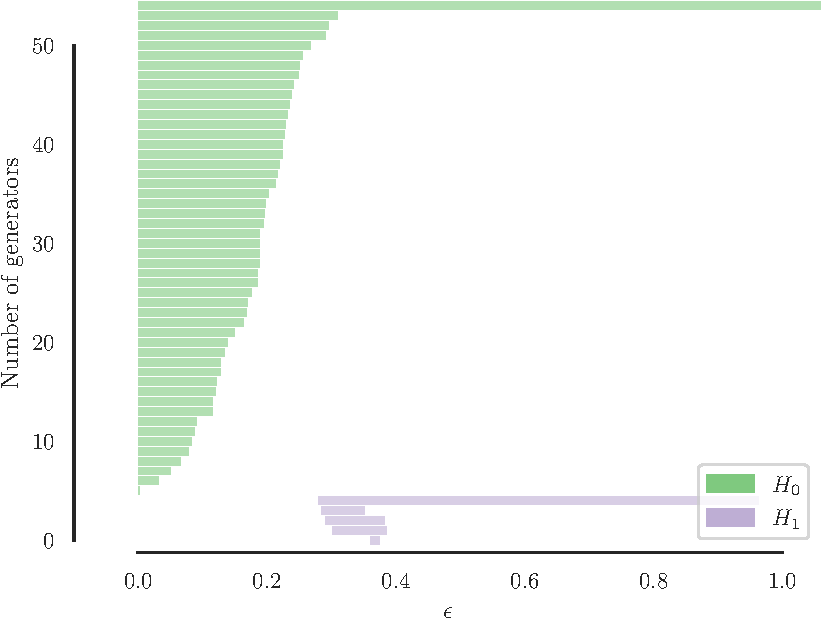
\includegraphics[scale=0.7]{barcode.pdf}};

\node[draw=black!100,line width=0.6mm, inner sep=0pt] (annulus0) at (-3.2,5.1)
    {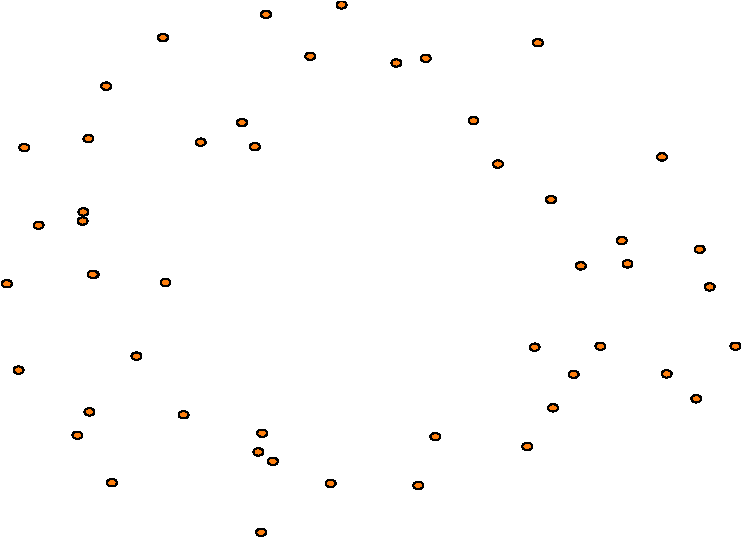
\includegraphics[scale=0.3]{annulus_eps0.pdf}};
    \draw[dotted,thick] (annulus0.south) -- (-3.2,-2.9);

\node[draw=black!100,line width=0.6mm, inner sep=0pt] (annulus3) at (-1,8)
    {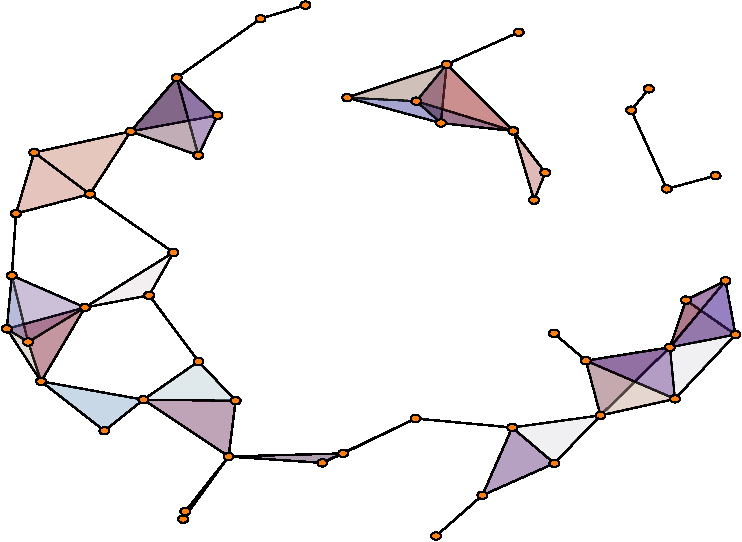
\includegraphics[scale=0.3]{annulus_eps3.pdf}};
\draw[dotted,thick] (annulus3.south) -- (-1,-2.9);

\node[draw=black!100,line width=0.6mm, inner sep=0pt] (annulus5) at (1.2,5.1)
    {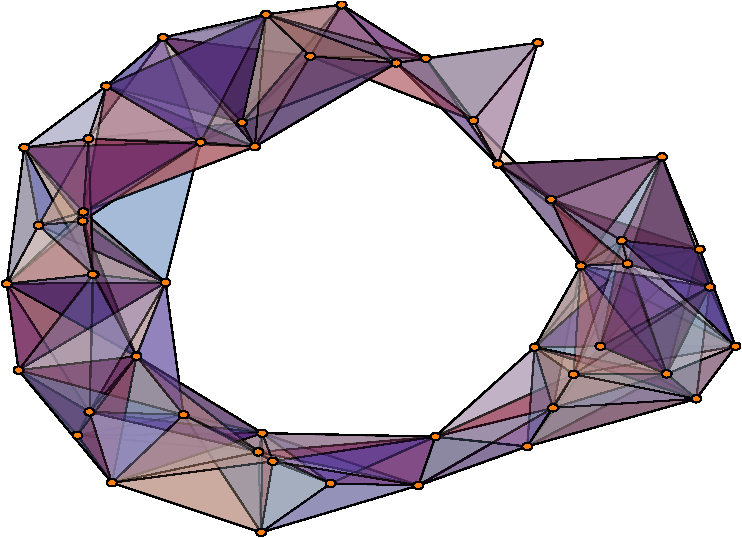
\includegraphics[scale=0.3]{annulus_eps5.pdf}};
    \draw[dotted,thick] (annulus5.south) -- (1.2,-2.9);
\node[draw=black!100,line width=0.6mm, inner sep=0pt] (annulus10) at (4.4,8)
    {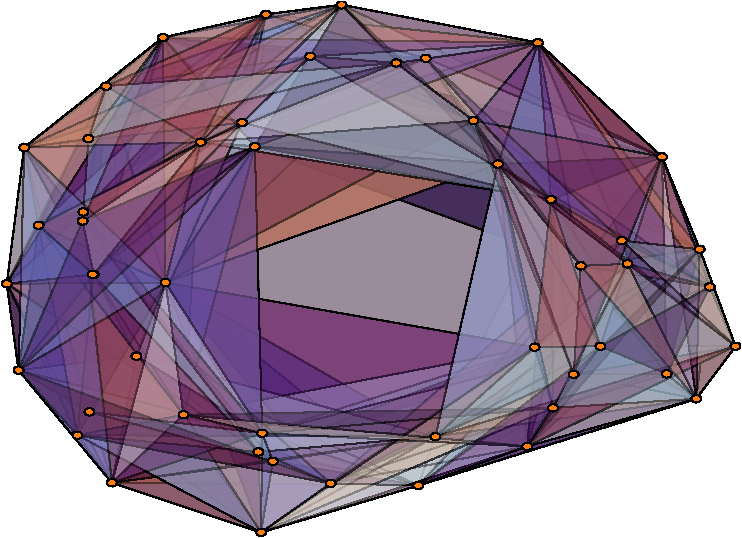
\includegraphics[scale=0.3]{annulus_eps10.pdf}};
\draw[dotted,thick] (annulus10.south) -- (4.4,-1.8);
\draw[dotted,thick] (4.4,-2.74) -- (4.4,-2.9);
\end{tikzpicture}
\caption{\label{annulus_barcode} Persistence barcode showing the birth and death of generators in the homology groups of a Vietoris-Rips complex approximated from points sampled from an annulus at different $\epsilon$. }
\end{figure}
  \subsection{Persistence Diagrams}
  Another way of illustrating persistent homology is the persistence diagram as seen in Figure \ref{pdiagram}. This is an alternative to the barcode in Figure \ref{annulus_barcode} where we instead plot the $\epsilon$-value on both axises and the further a point is from the diagonal line the longer the generator in the homology group survived. When we have a lot of birth-death pairs this is a preferable way of visualizing the persistent homology, since unlike the barcode it does not grow vertically with the number of generators.

  Just like in the barcode in Figure \ref{annulus_barcode} we can see that the only two generators that live for a considerable amount of time is a single connected component in $H_{0}$ and a single hole in $H_{1}$. This is consistent with the topology that we expect from an annulus.

  At around $\epsilon=0$ we see a lot of $H_{0}$ generators being born and dying after another. Since the number of generators of $H_{0}$ tells us the number of connected components in the topology this clearly illustrates how the sampled points go from being isolated islands to being incorporated in a larger simplex.
  \begin{figure}[ht]
    \centering
    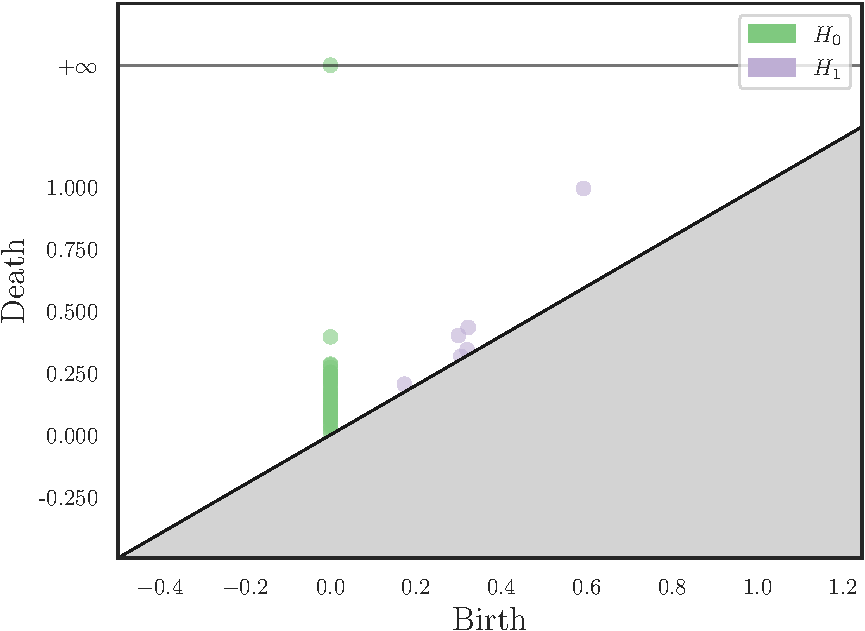
\includegraphics[scale=0.7]{diagram.pdf}
    \caption{\label{pdiagram} A persistence diagram over the birth and death of generators in the homology groups of a Vietoris-Rips complex approximated from points sampled from an annulus. The closer a point is to the diagonal line the shorter it lived. The diagram is truncated towards infinity, so generators that lived for a long enough time are considered to be at infinity.}
  \end{figure}

  \section{Metrics}
Given that we compute the persistent homology between two spaces, how can we compare them? There are two suitable metrics that are often used for doing this, namely the \textbf{q-Wasserstein distance} and the \textbf{Bottleneck distance}.
  \begin{definition}
    The Bottleneck distance between two persistence diagrams $X,Y$ is
    \[W_{\infty}(X,Y) = \inf_{\beta: X \to Y} \sup_{x \in X} ||x-\beta(x)||\]
  \end{definition}

  \begin{definition}
    The q-Wasserstein distance between two persistence diagrams $X,Y$ is
    \[W_{q}(X,Y) = (\inf_{\beta: X \to Y} \sum_{x \in X}  ||x-\beta(x)||^{q})^{\frac{1}{q}}\]
  \end{definition}
The Bottleneck distance is of particular interest since it gives a stability guarantee through the following theorem
  \begin{theorem}
    Given two filtering functions $f,g$ and a simplicial complex $K$ we have that
    \[W_{\infty}(f,g) \leq ||f-g||_{\infty}\]
  \end{theorem}
  In other words, any small perturbations of the filtering functions will at most be as large as the difference between the functions themselves.
\section{Computation of }
Some aspects of the computational part of this. How is it done in practice? Mention an example but do not dwell too much on this. Perhaps go into smith normal form and how it all translates to linear algebra?
%%% Local Variables:
%%% mode: latex
%%% TeX-master: "thesis.tex"
%%% End:
